%% In the derivation of the normal model, we assumed that $L\T m_3$, $L \T m_4$,
%% and $L \left( \T \right)^2 m_2$ go to zero as $L\to \infty$. The expectations of
%% the third and fourth moments thus go to zero as expected for a normal
%% distribution.

Deviations of the population distribution from normality depend on the
distribution of coalescent times and the genetic architecture, and they can be
investigated by comparison to the expected moments under normality. Even though
recombination is not included in the model, we can form an idea about how
linkage might impact deviations from normality. Line two of
equation \eqref{eq:emoms4} corresponds to the contribution from two mutations
occurring at a single locus. The first quantity indicates that the expectation
of the fourth moment increases with the variance of the pairwise coalescence
time. The second part does not have a clear interpretation. If the sum of these
two terms is positive this agrees with the intuition that linkage disequilibrium
increases deviations from normality by reducing the effective number of
independent loci.

When the mutation rate is low, the ratio of the expected fourth moment to that
under normality is
\begin{equation}
  \label{eq:popmom4coal}
  \frac{\E[M_4]}{3\left(L \T \E[\mathbbm{T}_{2,2}] m_2\right)^2} \approx 1 +
  \frac{m_2/m_4}{6 L \T \E[\mathbbm{T}_{2,2}]}\left( \frac{2\E[\mathbbm{T}_{4,4}] +
      \frac{2}{3}\E[\mathbbm{T}_{3,4}] +
      \frac{4}{9}\E[\mathbbm{T}_{2,4}]}{\E[\mathbbm{T}_{2,2}]}\right),
\end{equation}
The expected excess in $M_4$ is inversely related to the expected sparsity of
the trait which is proportional to $L \T \E[\mathbbm{T}_{2,2}]$. This excess
depends on demography through a factor $Q = \frac{2\E[\mathbbm{T}_{4,4}]
+ \frac{2}{3}\E[\mathbbm{T}_{3,4}]
+ \frac{4}{9}\E[\mathbbm{T}_{2,4}]}{\E[\mathbbm{T}_{2,2}]}$. The extent to which
demography increases or decreases deviations from normality can be investigated
by calculating $Q$ in different models. In a constant-size and panmictic
population $Q$ is equal to one. In a population where lineages are exchangeable,
$\E[\mathbbm{T}_{i,j}]$ can be calculated numerically using expressions from
\citet{Griffiths1998} or \citet{Polanski2003a}. Values of $Q$ in an exponentially growing population are
shown in Figure \ref{fig:Qexp}A. Holding sparsity and the mutational
distribution constant, a population which underwent exponential growth will have
a greater expected deviation from normality in its trait distribution. However,
the growth rate must exceed the present coalescent rate to increase $Q$ by more
than ten percent. Another useful example demography is a population that goes
through a step change at some point in the past. Figure \ref{fig:Qexp}B shows
that when the population size decreases looking into the past, $Q$ is increased
similarly to the exponential growth scenario. When the population size increases
looking into the past (a population bottleneck), $Q$ is decreased below one.
However, $Q$ appears more sensitive to population growth than to bottlenecks.

\begin{figure}
\centering
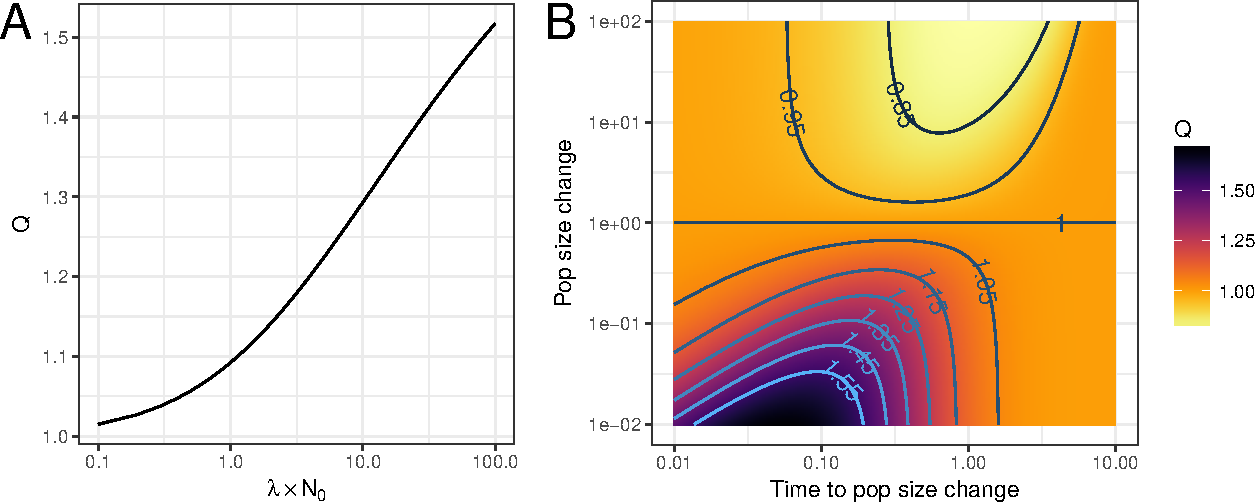
\includegraphics[width=\textwidth]{./figures/combo_q.pdf}

\caption{
\textbf{The effects of demography on deviations of the expected
fourth central moment of the population trait distribution for normality.} $Q$
measures the effect due to demography on the expected fourth central moment
(equation \eqref{eq:popmom4coal}). (\textbf{A}): $Q$ increases as the
exponential growth rate increases relative to the current population
size.~$\lambda$ is the growth rate and $N_0$ is the initial effective population
size.~(\textbf{B}): $Q$ values when the population undergoes an instantaneous
step change at some point in the past. The time and magnitude of this change are
given in units of the current effective population size. $Q$ increases when the
population grows and decreases when it declines. }

\label{fig:Qexp}
\end{figure}

\begin{figure}
\centering
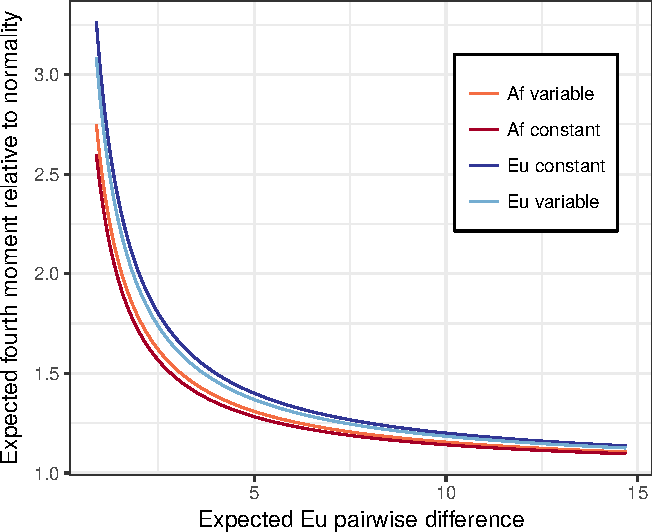
\includegraphics[width=0.55\textwidth]{./figures/af_eu_mom4_r.pdf}
\caption{ \textbf{A comparison between the expected fourth moment at different levels of
sparsity in the African and European demographic models fit
by \citet{Tennessen2012}.} Trait sparsity is varied by changing the expected
number pairwise differences at sites affecting the trait in the European model.
The mutational kurtosis is set to six. The darker lines show the predicted
relationship for populations with the same heterozygosity as the European and
African models but with constant size.}
\label{fig:afeucomp}
\end{figure}

As a concrete example, we can consider the differences in the expected fourth
moment produced by different demographic histories in different human
populations. In the demographic model fit by \citet{Tennessen2012}, the generic
European population experiences a bottleneck associated with out-of-Africa and
recent growth while the generic African population experiences a more stable
history also with recent growth. Differences in demographic history between the
two populations has resulted in a lower heterozygosity in European populations
due to the out-of-Africa bottleneck \citep{Yu2002}.

For a given sparsity, the African population model predicts a smaller deviation
from normality than the European model (Figure \ref{fig:afeucomp}). The expected
fourth moment in constant-size populations with the same heterozygosity as the
African and European models is lower for the African model and higher for the
European model. This is because the African model is dominated by population
growth that leads to a $Q$ greater than one, while the European model is
dominated by a bottleneck event that leads to a $Q$ less than one
(Figure \ref{fig:Qexp}). However, differences due to demography are small and
the overall deviations from normality are mostly driven by differences in
heterozygosity at causal loci.

Another natural way to quantify the deviation of a distribution from normality
is its kurtosis. The kurtosis, the ratio of the fourth central moment to the
square of the variance, measures the tendency of a distribution to produce
outliers \citep{Westfall2014}. Since the kurtosis of a trait distribution,
$\kappa_Y$, is ratio of two random quantities, its expectation is not
straightforward to calculate. A first order approximation to the kurtosis
suggests that $\kappa_Y$ will be greater than under normality when external
branches are longer and and less than under normality when they are longer
(Appendix \ref{kurtsim}).

However, simulations show that the first order approximation is very poor
(Figure \ref{fig:kurtsim}). The mean kurtosis increases when a trait becomes
sparse regardless of whether the population size is constant or growing.
Additionally, there is substantial variance in the kurtosis with about a quarter
of simulated populations having a kurtosis less than three even as the mean
kurtosis increases to almost nine. This high variance in the kurtosis is likely
due to a high variance in both the trait variance and fourth moment. This, along
with the fact that deviations from the infinitesimal model inflate the fourth
moment (equation \eqref{eq:popmom4coal}), leads to a situation where the
kurtosis increases with trait sparsity but the variance is high across
evolutionary realizations.

%%% Local Variables:
%%% TeX-master: "quant_gen_manu.tex"
%%% End:
